\section{AD Wandler \hartl{475}}

\subsection{Vergleich ADC}
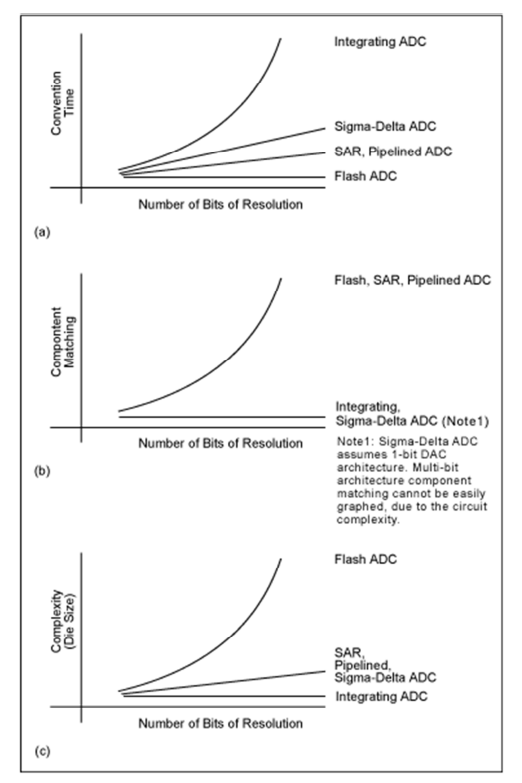
\includegraphics[width=9cm, valign=t]{pictures/vergleich_ADC.png}

\newpage

\subsection{Parallelverfahren und Kaskadenumsetzer}

\begin{longtable}{|>{\bfseries}p{4cm}|p{6cm}|p{8cm}|}
  \hline
    Parallelumsetzer (Flash-ADC) &
    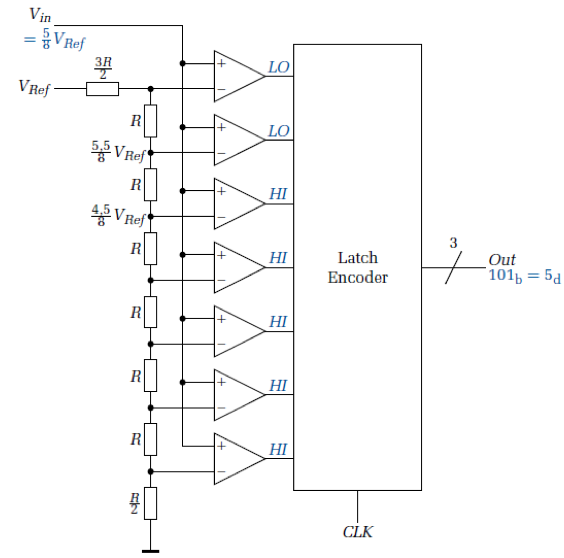
\includegraphics[width=6cm, valign=t]{pictures/parallelADC} &
    \begin{tabular}{ll}
      \textbf{Vorteile:} & sehr schnell \\
      & keine DAC Rückkopplung \\
      \textbf{Nachteile:} & geringe Auflösung \\
      & benötigt $2^n$ Widerstände \\
      & benötigt $2^n-1$ Komperatoren
    \end{tabular} \\
  \hline
    Kaskadenumsetzer (Pipeline ADC) &
    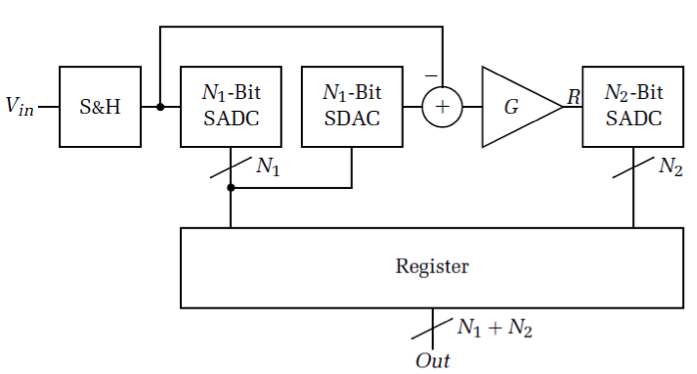
\includegraphics[width=6cm, valign=t]{pictures/kaskaden} \newline
    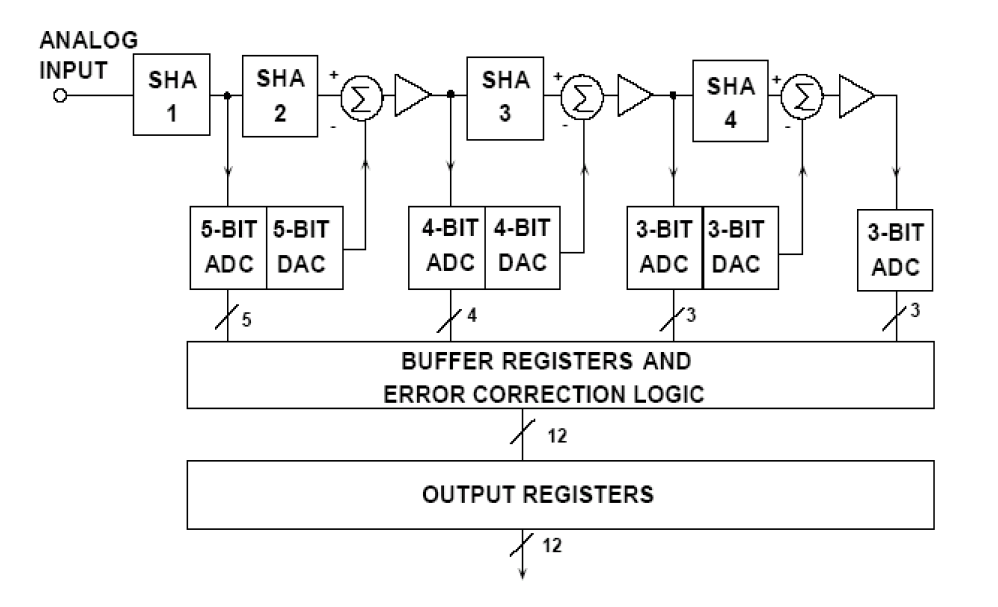
\includegraphics[width=6cm, valign=t]{pictures/kaskaden_fehlerkorrektur.png} \newline 
    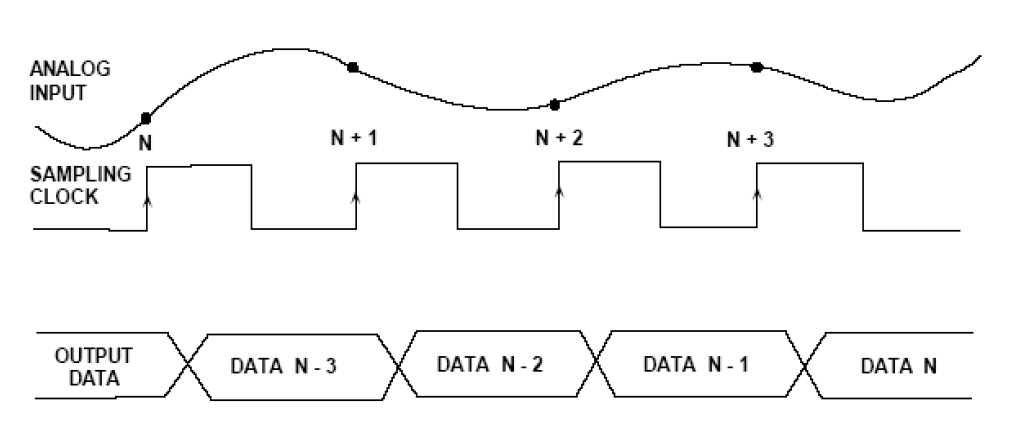
\includegraphics[width=6cm, valign=t]{pictures/latenz}&
    Eine 10-bit-Auflösung beim Parallelverfahren würde 1024 Komperatoren
    benötigen.$\Rightarrow$Komplexitätsreduktion \newline
    Mit erstem $N_{1}$-bit ADC wird der Grobbereich festgelegt (höherwertige
    Bits). Diese Zahl wird in eine analoge Spannung durch einen $N_{1}$-bit DAC zurück
    umgesetzt und diese Spannung von der Eingangsspannung subtrahiert. Diese
    Differenz wird von einem weiteren $N_{2}$-bit-ADC umgesetzt, um die
    niederwertigen Bits zu ergeben. Skaliert man die Differenzspannung mit dem
    Faktor 32, hat man den gleichen Spannungsbereich, kann also zwei identische
    ADC benutzen. \newline
    p = Anzahl Stufen \newline
    m = Bit pro Stufe \newline
    $p(2^m-1)$ Komperatoren \newline
    $n = p \cdot m$ \newline
    \newline
    \begin{tabular}{lp{6cm}}
      Bild 1: & Pipeline ADC ohne Fehlerkorrektur \\
      Bild 2: & Pipeline ADC mit Fehlerkorrektur \\
      Bild 3: & Verzögerung der Ausgangsdaten gegeüber den Sampels (Latenz)
    \end{tabular} \\
  \hline
\end{longtable}

\newpage

\subsection{Wägeverfahren (sukzessive Approximation/SAR) \hartl{485}}
\begin{longtable}{|>{\bfseries}p{4cm}|p{6cm}|p{8cm}|}
  \hline
    Prinip SAR &
    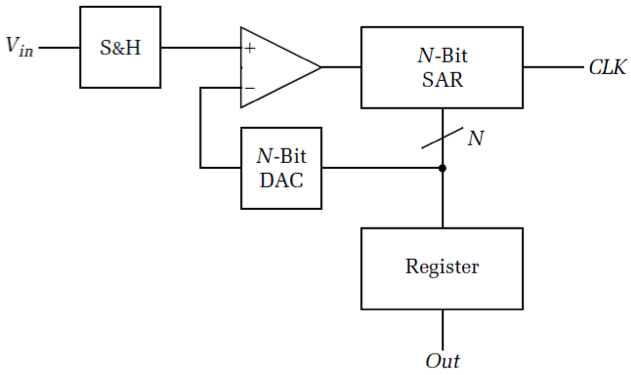
\includegraphics[width=6cm, valign=t]{pictures/waegeverfahren} &
    \begin{itemize}
      \item Abtastung der Eingangsspannung $V_{in}$mit einer
          S\&H-Schaltung( Vergleichsspannung liegt so während der gesamten
        Umsetzung an)
      \item Vergleich starte in der Mitte der Eingangsspannung $\frac{V_{Ref}}{2}$
    \end{itemize} \\
    
    &
    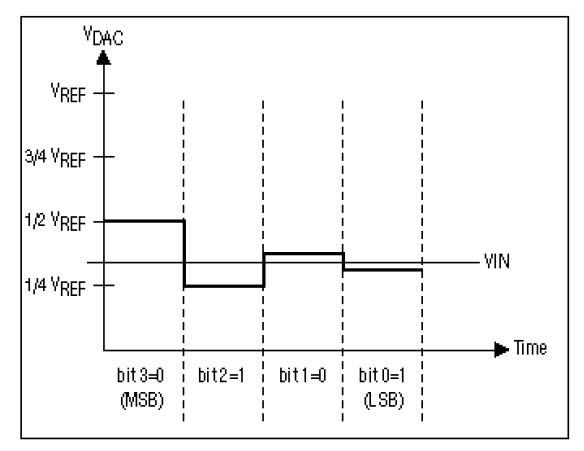
\includegraphics[width=6cm, valign=t]{pictures/prinzip_SAR.png} &
    \textbf{Ablauf der Wandlung:}
    \begin{enumerate}
      \item Im Sample-Hold wird ein analoger Wert gespeichert
      \item X(Laufvariable) wird auf n-1 gesetzt, DAC-Register wird auf 0 gsetzt
      \item Das Bit Bx vom DAC wird 1 gesetzt
      \item Komperator wird ausgewertet
            \begin{itemize}
              \item[1:] Bx = 1, DAC-Bit bleibt gesetzt
              \item[0:] Bx = 0, DAC-Bit wird gelöscht
            \end{itemize}
      \item X wird um 1 reduziert
      \item Gehe zu Schritt 3, wenn $X \geq 0$ 
    \end{enumerate} \\
  \hline
    Wägeverfahren mit SC-Prinzip &
    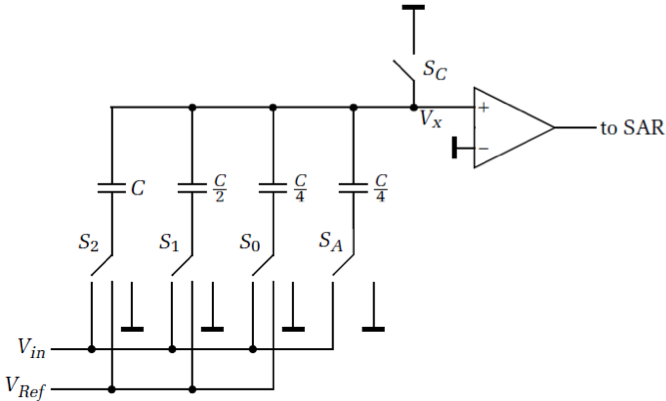
\includegraphics[width=6cm, valign=t]{pictures/waegeverfahrenSC} &
    \textbf{Ablauf der Wandlung:}
    \begin{enumerate}
      \item alle C mit $V_{in}$ laden
      \item $S_C$ öffnen
      \item $S_2, \ldots, S_A$ an $A_{GND}$
      \item Sukzessive $S_2, \ldots, S_0$ an $V_{Ref}$
    \end{enumerate}
    Wenn $S_2$ an $V_{Ref}$ ist gilt: $V_x = -V_{in}+\frac{V_{Ref}}{2}$ \newline
    Digitaler Wert $D = floor\left( \frac{V_{in}}{q}\right)$ \newline
    nicht aufgelöste Spannung: $V_{rest} = V_{in} \ mod \ q$\\
  \hline
\end{longtable}


\subsection{Iterative ADC}
\begin{longtable}{|p{12cm}|p{6cm}|}
  \hline
    \begin{enumerate}
      \item Im S/H wird die Eingangsspannung geschpeichert (Schalter Sin)
      \item Schalter Sin wird danach auf den Multiplizierer-Ausgang geschaltet
      \item X(Laufvariable) wird auf n-1 gesetzt
      \item Der Komparator wird ausgewertet\newline
        Dout=1: Bx=1, Switch S=1 (d.h. im Subtrahierer wird Vrefh von Vc
        subtrahiert)\newline
        Dout=0: Bx=0, Switch S=0 (d.h. im Subtrahierer wird 0 von Vc
        subtrahiert)
      \item Der Subtrahierer generiert sein Ausgangssignal
      \item Der Multiplizierer generiert sein Ausgangssignal
      \item Im S/H wird die Feedback-Spannung gespeichert (Schalter Sin)
      \item X wird um 1 reduziert
      \item Gehe zu Schritt 4, wenn $X\geq0$
    \end{enumerate} &
    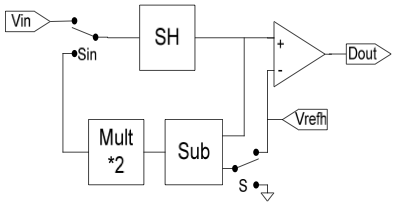
\includegraphics[width=6cm, valign=t]{pictures/iterativeADC}\newline
    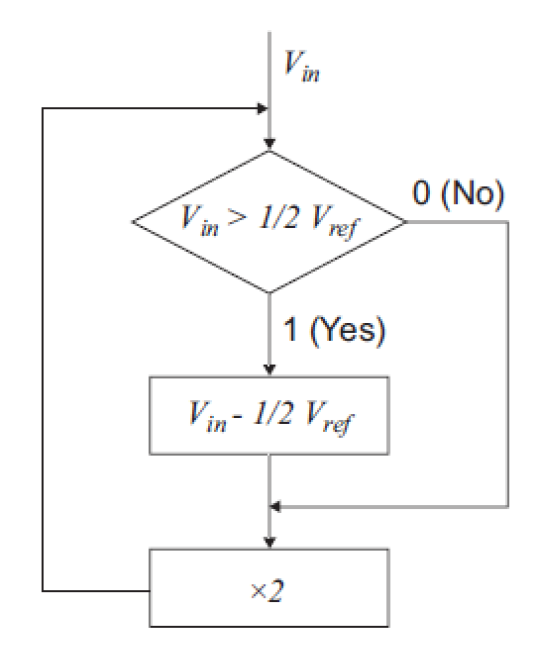
\includegraphics[width=6cm, valign=t]{pictures/iterativeADC_ablauf}\\
  \hline
\end{longtable}



\subsection{Zählverfahren \hartl{490}} 
Ist für kontinuierliche Auswertungen des Eingangssignal
\subsubsection{Single Slope}

\begin{tabular}{ccp{4cm}}
  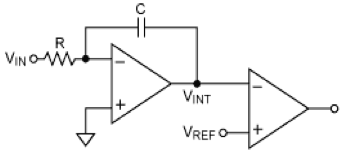
\includegraphics[width=6cm, valign=t]{pictures/singleSlope1} &
  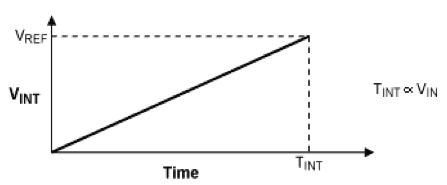
\includegraphics[width=6cm, valign=t]{pictures/singleSlope2} &
  {\begin{align*}
    V_{in}=\frac{V_{Ref} \cdot R \cdot C}{T_{int}}
  \end{align*}} \\
\end{tabular}

\subsubsection{Dual Slope \hartl{492}}
\begin{longtable}{cp{12cm}}
  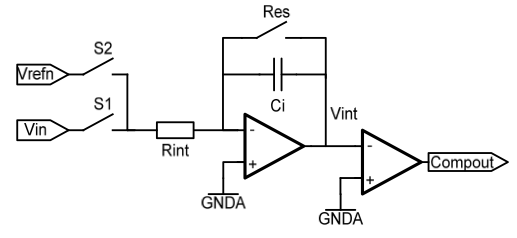
\includegraphics[width=6cm, valign=t]{pictures/dualSlope11} &
  $\begin{aligned}
 	T_{int} &= const \\
  	V_{int}(t) &= -\frac{1}{R_{int}\cdot C_i}\int_{0}^{t} (V_{in}(\tau) - V_{AGND})d\tau + V_{AGND}\\
   	V_{int}(T_{int}) &= V_{AGND} - \frac{1}{R_{int} \cdot C_i} \cdot T_{int} \cdot (V_{in} - V_{AGND}) \quad \textrm{(Für $V_{in}=$ const.)}\\
  \end{aligned}$\\
 
  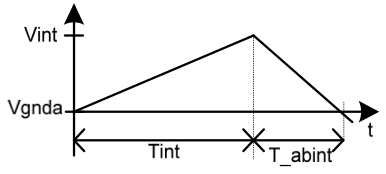
\includegraphics[width=6cm, valign=t]{pictures/dualSlope12} &
  \begin{tabular}{p{6cm}p{6cm}}
      \textbf{Integration:} &
      \textbf{Abintegration:} \\
  
      \[ V_{int_{max}} = - \dfrac{1}{R_i \cdot C_i} \cdot V_{in1} \cdot T_{int} \] &
      \[ V_{int}(t) = V_{int_{max}} - \dfrac{V_{Ref}}{R_i \cdot C_i}\cdot t \] 
  \end{tabular} \\
  
  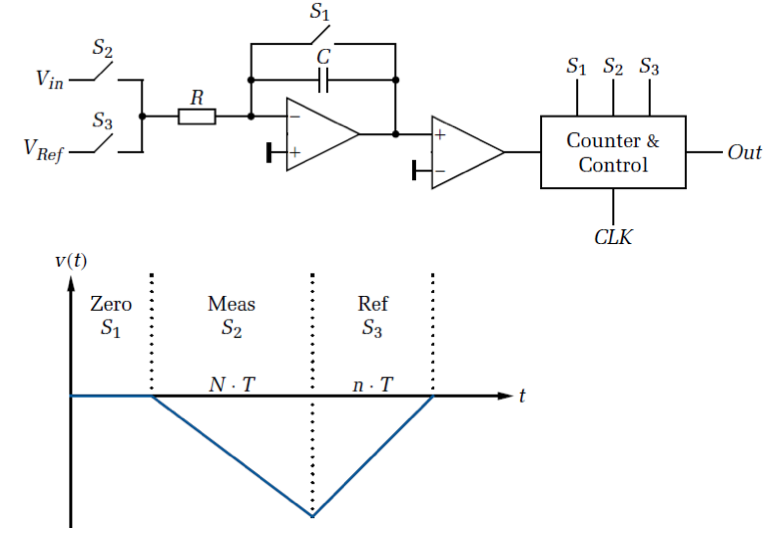
\includegraphics[width=6cm, valign=t]{pictures/dualSlope2} &
  \begin{tabular}{p{4cm}p{7cm}}
      \textbf{Abintegrationszeit:} &
      \textbf{Auflösung in Bits:} \\
  
      \[ t_{ab_{int}} = -\dfrac{V_{in1} \cdot T_{int}}{V_{Ref}} \] &
      \[ n = \dfrac{\log (\text{max Taktzyklen von Abintegration})}{\log(2)} \] 
  \end{tabular}
  \[ V_{in} = \frac{n}{N} \cdot V_{ref} \]
  
 Sinusschwingungen mit einer Periodendauer gleich der Integrationszeit, werden herausgefiltert!\\
 
  \begin{tabular}{ll}
    N:&Taktzyklen\\
    T:&Periodendauer\\
    n:&Zählerstand\\
    $V_{off}$:&Offsetspannung\\
  \end{tabular} &
  
  \begin{tabular}{ll}
    $T_{int}$:&Integrationszeit (ist vorgegeben)\\
    $T_{abint}$:& "`Messzeit"\\
    $V_{int}$:&Spannung am $V_{opOut}$ nach der Zeit $T_{int}$\\
    $V_{intmax}:$&maximal mögliche Spannung am $V_{opOut}$\\
  \end{tabular}
\end{longtable}

\begin{longtable}{p{4cm}p{6cm}p{8cm}}
  \textbf{Offsetkompensation:} &
  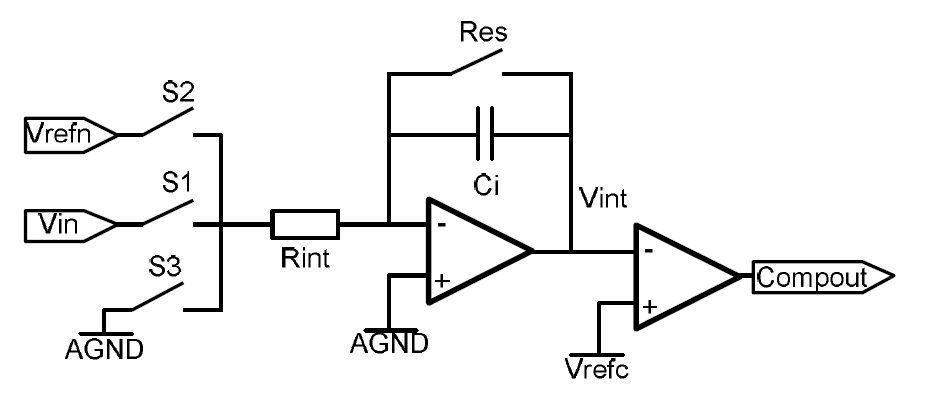
\includegraphics[width=6cm, valign=t]{pictures/offsetkompensation} &
  \textbf{Möglichkeiten zur Korrektur:}
  \begin{itemize}
    \item 2.Referenzspannung $V_{Refp}$ einfügen
    \item Die Komperator-Schwelle $V_{Refc}$ negativ gegeüber $AGND$ verschieben
    \item Dem OP einen Offset in einer Richtung vorgeben, damit er max 0 sein kann.
  \end{itemize}
\end{longtable}

\newpage

\subsubsection{Sigma-Delta Wandler \hartl{500}}
  \begin{longtable}{p{6cm}p{12cm}}
    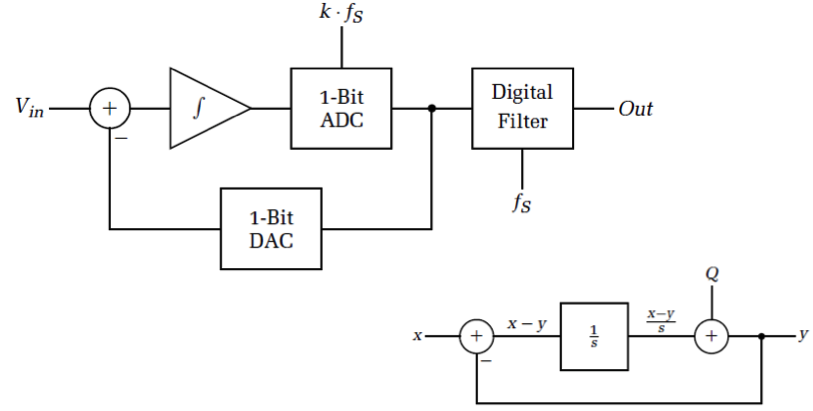
\includegraphics[width=6cm, valign=t]{pictures/deltaSigma1} \newline 
    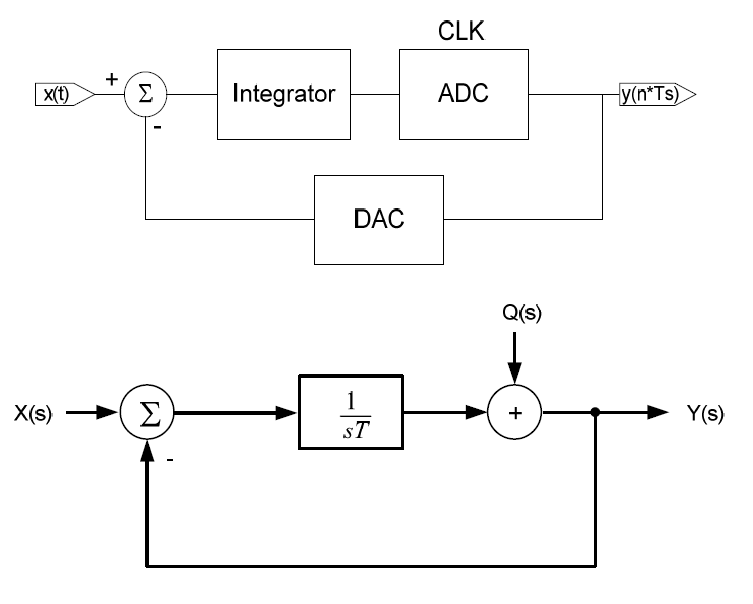
\includegraphics[width=6cm]{pictures/deltaSigma3} &
    \[Y=\frac{X-Y}{s}+Q\Rightarrow Y=X\frac{1}{1+s}+Q\frac{s}{1+s}\] \newline
    \begin{tabular}{p{3cm}p{9cm}}
      \textbf{Signal UTF:} &
      \textbf{Noise UTF:} \\
      
      \[ H_s(s) = \frac{1}{1+sT} \] &    
      \[ H_n(s) = \frac{sT}{1+sT} \] \\ \\
      
      SNR-Erhöhung: &
      $9dB$ oder 1.5Bit pro Verdoppelung des OSR (OverSamplingRatio) \\
      Hauptnachteil: &
      Pattern Noise (repetitive Sequenzen, die nicht von Signalen unterschieden werden können)
    \end{tabular}
    $Q(s)$ = Quantisierungsrauschen
    
  \end{longtable}

  %\begin{longtable}{cp{12cm}}
    %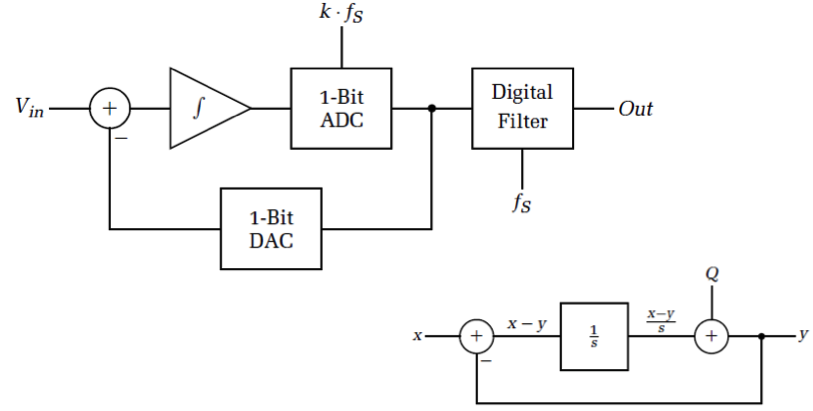
\includegraphics[width=6cm, valign=t]{pictures/deltaSigma1} &
    %\[Y=\frac{X-Y}{s}+Q\Rightarrow Y=X\frac{1}{1+s}+Q\frac{s}{1+s}\] \\
  %
    %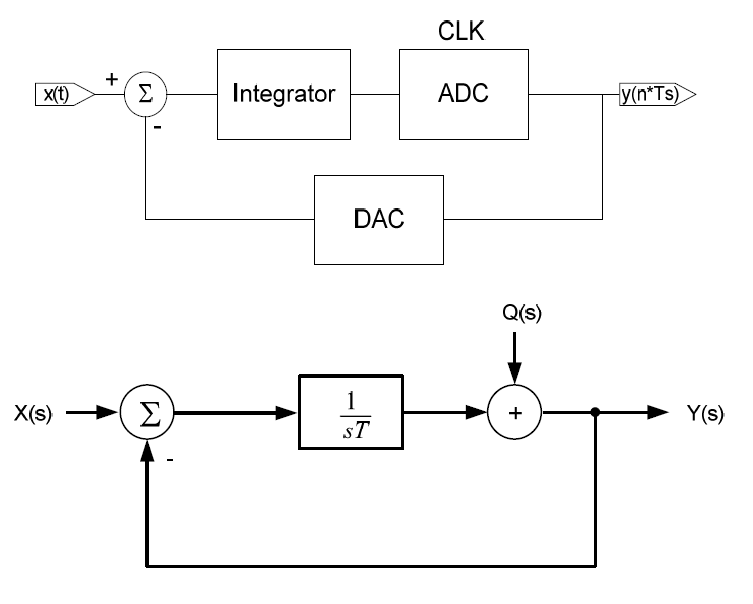
\includegraphics[width=6cm]{pictures/deltaSigma3} &
    %\begin{tabular}{p{3cm}p{9cm}}
      %\textbf{Signal UTF:} &
      %\textbf{Noise UTF:} \\
      %
      %\[ H_s(s) = \frac{1}{1+sT} \] &    
      %\[ H_n(s) = \frac{sT}{1+sT} \] \\ \\
      %
      %SNR-Erhöhung: &
      %$9dB$ oder 1.5Bit pro Verdoppelung des OSR (OverSamplingRatio) \\
      %Hauptnachteil: &
      %Pattern Noise (repetitive Sequenzen, die nicht von Signalen unterschieden werden können)
    %\end{tabular}
    %$Q(s)$ = Quantisierungsrauschen \newline
    %
  %\end{longtable}
	

%\subsubsection{Spannungs- Frequenz- Umsetzer \hartl{495}}
%\begin{multicols}{2}
	%\begin{center}
  		%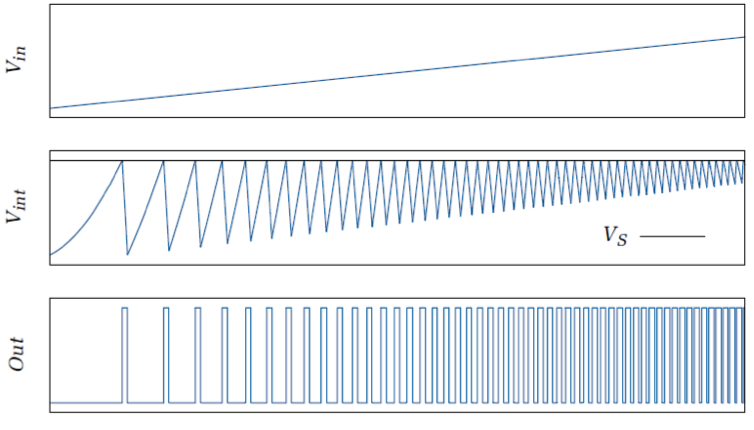
\includegraphics[width=7cm]{pictures/sfu_kurven}
  	%\end{center}
  %
  %
  %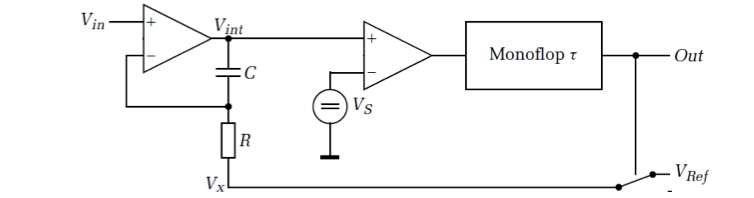
\includegraphics[width=6cm]{pictures/sfu_schaltung}
  %
   %\begin{align*}
      %V_{int}(t)=V_{in}+\frac{1}{RC}\int(V_{in}-V_{x})dt
   %\end{align*}
    %Vorteil: Immer am Eingangssignal\newline
    %Nachteil: Kein echter ADC  


%\subsubsection{Ladungs-Ausgleichs-Integrator \hartl{497}}
	%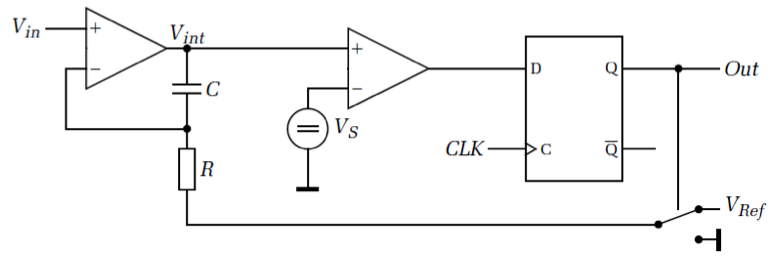
\includegraphics[width=6cm, valign=t]{pictures/lsg1} \\
	%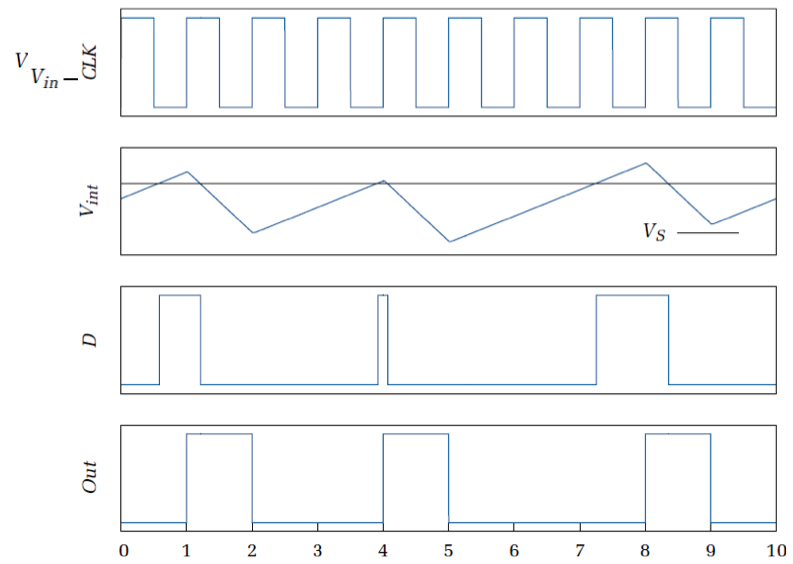
\includegraphics[width=6cm, valign=t]{pictures/lsg2}
	%\begin{itemize}
	   %\item Gleichgewichtsbedingung\\
	    %\begin{equation*}
	      %V_{in}-\frac{n}{N}V_{Ref}=0\Rightarrow n=\frac{V_{in}}{V_{Ref}}N
	    %\end{equation*}
	  %\item Flipflop statt Monoflop
	%\end{itemize}
%\end{multicols}	

\begin{multicols}{2}
  \subsubsection{Sigma-Delta Wandler 2. Ordnung}
    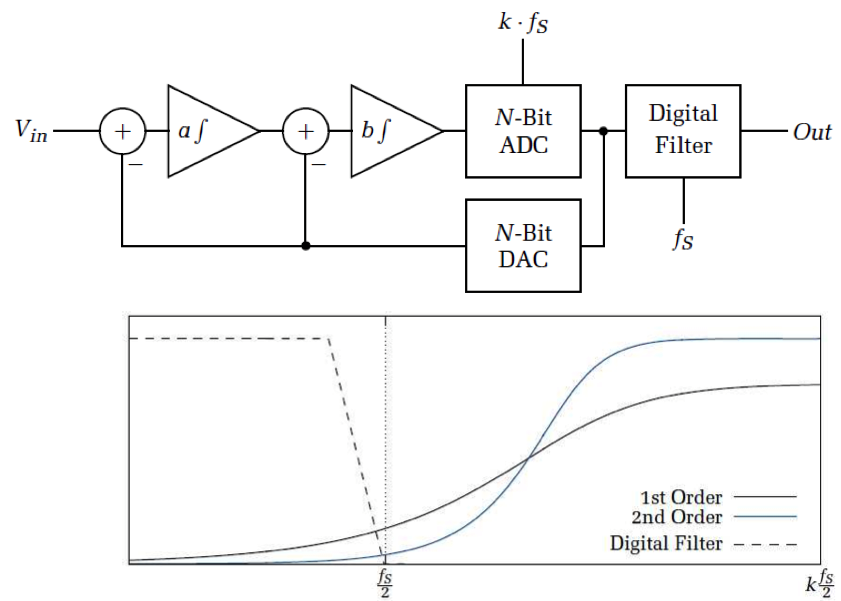
\includegraphics[width=6cm, height =4cm]{pictures/deltaSigma2}
  
  \columnbreak
  
  \subsubsection{PWM vs. Sigma-Delta}
      \textbf{Digitalteil PWM}
      \begin{itemize}
        \item Zähler zählt bis $2^n$
        \item Komperator schaltet Ausgang
        \item '1' sind hintereinander
      \end{itemize}
      
      \textbf{Digitalteil Sigma-Delta DAC}
      \begin{itemize}
        \item Dig.wert wird "`integriert"'
        \item Übertrag schaltet Ausgang
        \item '1' werden verteilt
      \end{itemize}
\end{multicols}

\subsection{Dynamikbereich}
\subsubsection{Dithering}
  Ein Signal kann mittel Mittelwertbildung höher aufgelöst werden, wenn es mit Rauschen überlager ist.
  Die Auflösung wird gegen Bandbreite "`eingetauscht"' (Die Rauschleistung wird auf die Bandbreite aufgeteilt,
  dadurch ist nur noch ein kleiner Rauschanteil im Signalband).
  
\subsubsection{Oversampling}
  \begin{tabular}{lll}
    Over Sampling Ratio: &
    $OSR = \dfrac{f_s}{2+f_{max}}$ & \\
    
    Signal to Noise Ratio: &
    $SNR_{dB} = 1.76dB + n \cdot 6.02dB$ &
    (ohne Überabtastung)\\
    
    & $SNR_{dB} = 1.76dB + n \cdot 6.02dB + 10 \cdot \log (OSR)$ &
    (mit Überabtastung)
  \end{tabular}
  
  Durch Überabtastung wird das Quantisierungsrauschen über einen grösseren Frequenzbereich verteilt.
  Da die Rauschleistungsdichte ($=q^2/12$) konstant ist, wird durch eine grössere Bandbreite die
  Rauschleistungsdichte kleiner.
  
\subsubsection{Effektive Bit-Zahl (ENOB)}
  \begin{tabular}{lp{8cm}}
    Signal to Noise and Distortion: &
    \[SINAD = 10 \cdot \log \left(\dfrac{P_{signal}+P_{noise}+P_{distortion}}{P_{noise}+P_{distortion}}\right)\] \\
    Effective Number of Bits: &
    \[ENOB = \dfrac{SINAD-1.76}{6.02}\]
  \end{tabular}

  
  


